\documentclass[aspectratio=169]{beamer}

\usetheme{Boadilla}
\usefonttheme{professionalfonts}
\setbeamertemplate{navigation symbols}{}
\setbeamertemplate{itemize items}[circle]
\setbeamertemplate{enumerate items}[default]
\setbeamertemplate{headline}{}

\usepackage[utf8]{inputenc}
\usepackage[T1]{fontenc}
\usepackage{lmodern}
\usepackage{amsmath}
\usepackage{booktabs}
\usepackage{tabularx}
\usepackage{array}
\usepackage{hyperref}
\usepackage[strings]{underscore}
\usepackage{listings}
\usepackage{tikz}
\usetikzlibrary{arrows.meta,positioning,fit,calc,shapes.geometric}
\usepackage{xcolor}

\definecolor{courseblue}{HTML}{12355B}
\definecolor{coursegold}{HTML}{C98A2E}
\definecolor{courseice}{HTML}{EEF3F8}
\definecolor{coursegreen}{HTML}{2F6B4F}
\definecolor{coursegray}{HTML}{4B5563}
\definecolor{codebg}{HTML}{F7F9FC}
\definecolor{codecomment}{HTML}{5E6C84}
\definecolor{codestring}{HTML}{0B6E4F}

\setbeamercolor{palette primary}{bg=courseblue,fg=white}
\setbeamercolor{palette secondary}{bg=coursegold,fg=white}
\setbeamercolor{palette tertiary}{bg=courseblue,fg=white}
\setbeamercolor{palette quaternary}{bg=coursegold,fg=white}
\setbeamercolor{structure}{fg=courseblue}
\setbeamercolor{frametitle}{bg=courseice,fg=courseblue}
\setbeamercolor{title}{fg=courseblue}
\setbeamercolor{block title}{bg=courseblue,fg=white}
\setbeamercolor{block body}{bg=courseice,fg=black}
\setbeamercolor{normal text}{fg=black,bg=white}
\setbeamercolor{alerted text}{fg=coursegold}

\setbeamerfont{footline}{size=\scriptsize}

\setbeamertemplate{footline}{
  \leavevmode
  \hbox{
    \begin{beamercolorbox}[wd=.33\paperwidth,ht=2.8ex,dp=1.2ex,leftskip=0.8em]{palette primary}%
      University of Trieste
    \end{beamercolorbox}%
    \begin{beamercolorbox}[wd=.49\paperwidth,ht=2.8ex,dp=1.2ex,center]{palette tertiary}%
      \coursename{} \textbar{} \coursecode
    \end{beamercolorbox}%
    \begin{beamercolorbox}[wd=.18\paperwidth,ht=2.8ex,dp=1.2ex,rightskip=0.8em plus1fil]{palette secondary}%
      \insertframenumber{} / \inserttotalframenumber
    \end{beamercolorbox}%
  }
}

\hypersetup{
  colorlinks=true,
  linkcolor=courseblue,
  urlcolor=coursegreen
}

\lstdefinestyle{coursepython}{
  language=Python,
  basicstyle=\ttfamily\footnotesize,
  keywordstyle=\color{courseblue}\bfseries,
  commentstyle=\color{codecomment}\itshape,
  stringstyle=\color{codestring},
  showstringspaces=false,
  columns=fullflexible,
  keepspaces=true,
  frame=single,
  framerule=0.6pt,
  rulecolor=\color{courseblue},
  backgroundcolor=\color{codebg},
  xleftmargin=0.4em,
  xrightmargin=0.4em,
  aboveskip=0.4em,
  belowskip=0.2em
}

\newcommand{\coursename}{Data-driven Systems Engineering}
\newcommand{\coursecode}{440MI / 305SM}
\newcommand{\coursefooter}{}

\newcommand{\learninggoals}[1]{
  \begin{block}{Learning goals}
  #1
  \end{block}
}

\newcommand{\repoactivity}[1]{
  \begin{block}{Repo activity}
  #1
  \end{block}
}

\newcommand{\readinglist}[1]{
  \begin{block}{Papers and materials}
  {\footnotesize #1}
  \end{block}
}

\newcommand{\coursecontextframe}[5]{
  \begin{frame}{Course Map and Running Cases}
  \centering
  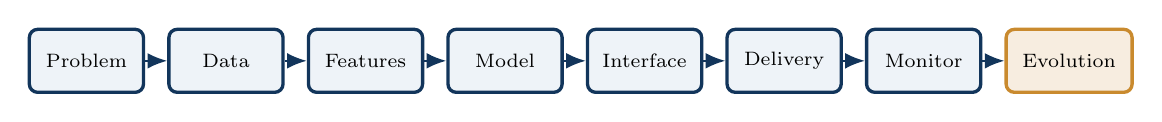
\begin{tikzpicture}[node distance=0.28cm]
  \node[flowbox, minimum width=1.45cm, minimum height=0.8cm] (problem) {\scriptsize Problem};
  \node[flowbox, minimum width=1.45cm, minimum height=0.8cm, right=of problem] (data) {\scriptsize Data};
  \node[flowbox, minimum width=1.45cm, minimum height=0.8cm, right=of data] (features) {\scriptsize Features};
  \node[flowbox, minimum width=1.45cm, minimum height=0.8cm, right=of features] (model) {\scriptsize Model};
  \node[flowbox, minimum width=1.45cm, minimum height=0.8cm, right=of model] (interface) {\scriptsize Interface};
  \node[flowbox, minimum width=1.45cm, minimum height=0.8cm, right=of interface] (delivery) {\scriptsize Delivery};
  \node[flowbox, minimum width=1.45cm, minimum height=0.8cm, right=of delivery] (monitor) {\scriptsize Monitor};
  \node[accentbox, minimum width=1.6cm, minimum height=0.8cm, right=of monitor] (evolution) {\scriptsize Evolution};
  \foreach \a/\b in {problem/data,data/features,features/model,model/interface,interface/delivery,delivery/monitor,monitor/evolution} {
    \draw[arrow] (\a) -- (\b);
  }
  \end{tikzpicture}

  \vspace{0.5em}
  \begin{block}{Today in the course}
  \textbf{Focus:} #1

  \textbf{Bridge:} #2
  \end{block}

  \begin{columns}[T]
  \column{0.48\textwidth}
  \begin{block}{Fraud case}
  {\footnotesize #3}
  \end{block}
  \column{0.48\textwidth}
  \begin{block}{Pasteurization case}
  {\footnotesize #4}
  \end{block}
  \end{columns}

  \vspace{0.3em}
  {\footnotesize \textbf{Course thread:} #5}
  \coursefooter
  \end{frame}
}

\newcommand{\classclosingframe}[4]{
  \begin{frame}{From This Class to the Next}
  \begin{block}{What stays with us}
  #1
  \end{block}

  \begin{columns}[T]
  \column{0.48\textwidth}
  \begin{block}{Project use}
  {\footnotesize #2}
  \end{block}
  \column{0.48\textwidth}
  \begin{block}{Next connection}
  {\footnotesize #3}
  \end{block}
  \end{columns}

  \vspace{0.3em}
  {\footnotesize \textbf{Course thread:} #4}
  \coursefooter
  \end{frame}
}

\tikzset{
  flowbox/.style={
    rounded corners=3pt,
    draw=courseblue,
    fill=courseice,
    very thick,
    minimum width=2.2cm,
    minimum height=0.9cm,
    align=center,
    font=\small
  },
  accentbox/.style={
    rounded corners=3pt,
    draw=coursegold,
    fill=coursegold!15,
    very thick,
    minimum width=2.2cm,
    minimum height=0.9cm,
    align=center,
    font=\small
  },
  arrow/.style={
    -{Latex[length=2.5mm,width=2mm]},
    thick,
    draw=courseblue
  }
}


\title{Class 15: Model Monitoring and Drift Response}
\author{\coursename}
\date{}

\begin{document}

\frame{\titlepage \coursefooter}

\begin{frame}{Agenda}
\begin{itemize}
\item Why monitoring matters
\item Monitoring as risk control
\item Monitoring types
\item Data drift versus concept drift
\item Detection strategies
\item Performance over time and business metrics
\item Response after alerts
\end{itemize}
\coursefooter
\end{frame}

\begin{frame}{Monitoring turns deployment into a feedback loop}
\learninggoals{
\begin{itemize}
\item Distinguish system, data, model, and business monitoring layers.
\item Compare data drift, concept drift, and pipeline failure symptoms.
\item Design practical responses after a drift alert.
\item Explain why monitoring starts before deployment rather than after it.
\end{itemize}
}
\coursefooter
\end{frame}

\coursecontextframe
{Monitoring, drift response, and system evolution.}
{This final class closes the lifecycle by showing how deployed systems remain trustworthy after release and how change feeds back into new work.}
{In the fraud case, monitoring covers data shift, score behavior, analyst workload, and the cost of false alerts over time.}
{In the pasteurization case, monitoring covers sensor quality, state transitions, prediction error, and when a drift alert should trigger investigation or retraining.}
{The course ends where real systems live: not at deployment, but in continuous observation, response, and evolution.}

\begin{frame}{Why monitoring matters}
\begin{itemize}
\item ML systems are data products, not static binaries.
\item Degradation can be silent and expensive.
\item Labels may arrive late, so proxies matter.
\item Monitoring is evidence for operations, governance, and improvement.
\end{itemize}
\coursefooter
\end{frame}

\begin{frame}{Monitoring is quantified risk management}
\begin{itemize}
\item Data risk: changed distributions, missing features, schema violations.
\item Model risk: degraded performance, instability, concept drift, unfairness.
\item Operational risk: broken pipelines, latency spikes, failed endpoints.
\item Business risk: review overload, poor intervention yield, loss of trust.
\end{itemize}
\begin{block}{Meaning}
Monitoring turns hidden failure into visible evidence that teams can act on.
\end{block}
\coursefooter
\end{frame}

\begin{frame}{What should be monitored in an ML service?}
\centering
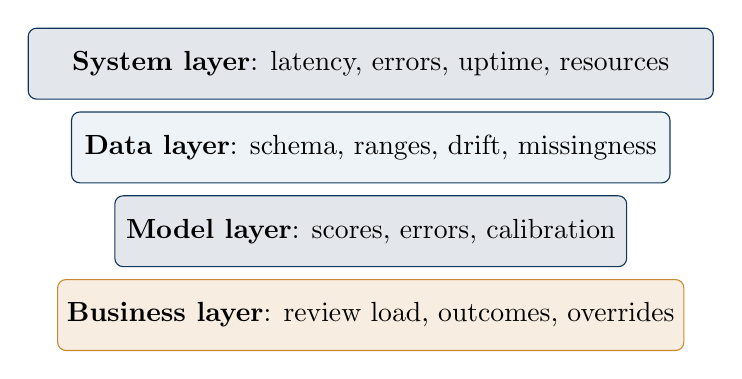
\begin{tikzpicture}[node distance=0.15cm]
\node[draw=courseblue, fill=courseblue!12, rounded corners=3pt, minimum width=8.7cm, minimum height=0.9cm] (system) {\textbf{System layer}: latency, errors, uptime, resources};
\node[draw=courseblue, fill=courseice, rounded corners=3pt, minimum width=7.6cm, minimum height=0.9cm, below=of system] (data) {\textbf{Data layer}: schema, ranges, drift, missingness};
\node[draw=courseblue, fill=courseblue!12, rounded corners=3pt, minimum width=6.5cm, minimum height=0.9cm, below=of data] (model) {\textbf{Model layer}: scores, errors, calibration};
\node[draw=coursegold, fill=coursegold!15, rounded corners=3pt, minimum width=5.4cm, minimum height=0.9cm, below=of model] (biz) {\textbf{Business layer}: review load, outcomes, overrides};
\end{tikzpicture}
\coursefooter
\end{frame}

\begin{frame}{Classical monitoring versus ML monitoring}
\begin{columns}[T]
\column{0.48\textwidth}
\textbf{Traditional systems}
\begin{itemize}
\item CPU, memory, disk
\item Request rate and latency
\item Availability and error codes
\end{itemize}
\column{0.48\textwidth}
\textbf{ML systems add}
\begin{itemize}
\item Feature quality and schema checks
\item Drift and score shifts
\item Delayed labels and performance decay
\end{itemize}
\end{columns}
\coursefooter
\end{frame}

\begin{frame}{Data drift vs concept drift}
\begin{itemize}
\item Data drift: input distribution changes, even if the relationship still holds.
\item Concept drift: the mapping from input to target changes.
\item Pipeline bugs can mimic both and must be ruled out early.
\end{itemize}
\begin{block}{Examples}
Holiday shopping patterns can cause fraud feature drift; a new attack strategy can create concept drift.
\end{block}
\coursefooter
\end{frame}

\begin{frame}{What can look like drift but is not}
\begin{itemize}
\item A broken ingestion job that changes missing-value rates.
\item A schema change that reorders or renames columns.
\item A deployment mismatch between training preprocessing and live preprocessing.
\item A monitoring bug that changes the way metrics are computed.
\end{itemize}
\begin{block}{Rule}
Before retraining, verify that the problem is real and not a pipeline defect.
\end{block}
\coursefooter
\end{frame}

\begin{frame}{Detection strategies}
\begin{itemize}
\item Batch statistical tests: KS, PSI, chi-square, Jensen-Shannon variants.
\item Prediction monitoring: score distribution and confidence shifts.
\item Label-based metrics when ground truth arrives.
\item Streaming detectors: ADWIN, Page-Hinkley, DDM, EDDM.
\end{itemize}
\coursefooter
\end{frame}

\begin{frame}{A practical drift-detection taxonomy}
\begin{tabularx}{\textwidth}{>{\bfseries}l X}
Signal type & Typical use \\
\toprule
Feature distribution tests & Early warning when labels are delayed. \\
Prediction distribution checks & Detect score collapse or threshold instability. \\
Label-based performance & Confirm concept drift when outcomes arrive. \\
Streaming detectors & Catch online change in error or metric sequences. \\
Segment analysis & Reveal that drift affects only some populations. \\
\bottomrule
\end{tabularx}
\coursefooter
\end{frame}

\begin{frame}[fragile]{Repository-style online monitoring loop}
\begin{lstlisting}[style=coursepython]
y_pred = model.predict_one(x)
model.learn_one(x, y)
mae.update(y, y_pred)
error = abs(y - (y_pred or 0))
adwin.update(error)
drift_flag = adwin.drift_detected
\end{lstlisting}
\begin{itemize}
\item `streamlit/pages/App_Stream.py` uses this pattern to combine incremental learning, error tracking, and ADWIN-based change detection.
\item It is useful because the alert is tied to live behavior, not only offline charts.
\end{itemize}
\coursefooter
\end{frame}

\begin{frame}{Repo examples for a stronger lecture}
\repoactivity{
\begin{itemize}
\item `streamlit/pages/App_Stream.py` already combines online learning with ADWIN.
\item `documents/Forecasting_and_Drift_Pasteurization.pdf` defines a project around forecasting and drift detection.
\item `pasteurization/synth_sensors.py` gives state-aware signals for meaningful monitoring discussions.
\end{itemize}
}
\coursefooter
\end{frame}

\begin{frame}{Labels arrive late, so proxies become important}
\begin{itemize}
\item In many real systems, ground truth appears hours, days, or weeks later.
\item Teams therefore monitor proxies such as score distribution, alert rate, abstentions, or operator overrides.
\item Proxy metrics are not substitutes for truth, but they reduce blind spots between retraining cycles.
\end{itemize}
\coursefooter
\end{frame}

\begin{frame}{What to do after detection}
\begin{enumerate}
\item Verify the alert is not caused by ingestion or schema issues.
\item Diagnose whether the change is temporary, seasonal, or structural.
\item Choose a response: retrain, recalibrate, switch model, or escalate to humans.
\item Record the event for later audit and process learning.
\end{enumerate}
\coursefooter
\end{frame}

\begin{frame}{Typical responses after a monitoring event}
\begin{itemize}
\item Retrain when the environment has genuinely shifted and new labels are available.
\item Recalibrate when confidence is wrong but ranking remains useful.
\item Roll back when a release introduced the failure.
\item Add human review when uncertainty is high and automated action is risky.
\item Change thresholds when business cost trade-offs have shifted.
\end{itemize}
\coursefooter
\end{frame}

\begin{frame}{Performance over time and business metrics}
\begin{itemize}
\item Model metrics: accuracy, precision, recall, AUC, MAE, RMSE.
\item Operational metrics: latency, queue length, failed predictions.
\item Business metrics: intervention yield, review load, false alert fatigue.
\item Human signals: overrides, complaints, and trust breakdowns.
\end{itemize}
\coursefooter
\end{frame}

\begin{frame}{Champion-challenger and continuous comparison}
\begin{itemize}
\item A champion model serves production traffic.
\item A challenger runs in shadow mode or on sampled traffic.
\item Comparison over time helps avoid switching on the basis of one lucky offline result.
\item This strategy is especially useful when concept drift is suspected but labels are delayed.
\end{itemize}
\coursefooter
\end{frame}

\classclosingframe
{\begin{itemize}
\item Monitoring turns deployment into an ongoing feedback process instead of an endpoint.
\item Drift detection matters only when the team has diagnosis and response mechanisms.
\item The full course lifecycle closes here: systems must evolve as data, users, and risks change.
\end{itemize}}
{For both running cases, long-term value depends on observing data quality, model behavior, operational health, and human consequences over time.}
{This closing class links back to the first one: every architecture, feature, model, interface, and process choice should support sustainable evolution.}
{The course ends with the same systems view it began with, now grounded in concrete engineering practices across the whole lifecycle.}

\begin{frame}{Papers and materials}
\readinglist{
\href{https://riverml.xyz/latest/api/drift/ADWIN/}{River ADWIN documentation};\ 
\href{https://www.oreilly.com/library/view/practical-mlops/9781098103002/}{Practical MLOps};\ 
\href{https://www.oreilly.com/library/view/reliable-machine-learning/9781098106218/}{Reliable Machine Learning};\ 
\href{https://arxiv.org/abs/2007.06299}{Gama et al., A survey on concept drift adaptation};\ 
\href{https://evidentlyai.com/blog/data-drift-detection-large-datasets}{Evidently on data drift detection};\ 
\href{https://prometheus.io/docs/introduction/overview/}{Prometheus monitoring overview}.
}
\coursefooter
\end{frame}

\end{document}
